\documentclass[format=acmsmall, review=false, screen=true]{acmart}

\usepackage{booktabs} % For formal tables
\usepackage{lipsum}

\usepackage[utf8]{inputenx}
\usepackage[T1]{fontenc} % Codificación de salida 

\usepackage{subcaption} % Used for subfigure

\usepackage[ruled]{algorithm2e} % For algorithms
\renewcommand{\algorithmcfname}{ALGORITHM}
\SetAlFnt{\small}
\SetAlCapFnt{\small}
\SetAlCapNameFnt{\small}
\SetAlCapHSkip{0pt}
\IncMargin{-\parindent}


% Metadata Information
%\acmJournal{TWEB}
%\acmVolume{9}
%\acmNumber{4}
%\acmArticle{39}
%\acmYear{2018}
%\acmMonth{3}
%\copyrightyear{2018}
%\acmArticleSeq{9}

% Copyright
%\setcopyright{acmcopyright}
%\setcopyright{acmlicensed}
%\setcopyright{rightsretained}
%\setcopyright{usgov}
%\setcopyright{usgovmixed}
%\setcopyright{cagov}
%\setcopyright{cagovmixed}

% DOI
\acmDOI{0000001.0000001}


% Document starts
\begin{document}
	% Title portion. Note the short title for running heads
	\title{Sistema de predicción de retrasos en vuelos}
	
	\author{Fernando Vallejo}
	\affiliation{%
		\institution{Universidad de Castilla-La Mancha}
		\city{Ciudad Real}
		\state{Ciudad Real}
		\country{Spain}
	}
	\email{Fernando.Vallejo@alu.uclm.es}
	\author{Juan José Corroto}
	\affiliation{%
		\institution{Universidad de Castilla-La Mancha}
		\city{Ciudad Real}
		\state{Ciudad Real}
		\country{Spain}
	}
	\email{JuanJose.Corroto@alu.uclm.es}
	\author{Alvaro Guerrero}
	\affiliation{%
		\institution{Universidad de Castilla-La Mancha}
		\city{Ciudad Real}
		\state{Ciudad Real}
		\country{Spain}
	}
	\email{Alvaro.Guerrero1@alu.uclm.es}
	\author{Javier Cordoba}
	\affiliation{%
		\institution{Universidad de Castilla-La Mancha}
		\city{Ciudad Real}
		\state{Ciudad Real}
		\country{Spain}
	}
	\email{Javier.Cordoba1@alu.uclm.es}
	
\maketitle

\begin{abstract}
	\lipsum[1]
\end{abstract}

\keywords{KDD Process, Mineria de datos}

\section{Introducción}

\section{Proceso KDD}
\subsection{Selección}
\subsection{Preproceso}
\subsection{Transformation}
\subsection{Minería de Datos (Primera Aproximación)}
En esta primera aproximación realizaremos una clasificación binaria de forma que intentaremos predecir cuando un vuelo se va a retrasar (1) o no (0), en base a los datos que sabemos a priori en un vuelo. En este caso, usaremos los siguientes datos:
\begin{itemize}
	\item El nombre de la aerolínea encargada del vuelo.
	\item El día de verano, es decir, dentro de la temporada del verano (Junio, Julio y Agosto), en qué día nos situamos.
	\item Hora programada de salida.
	\item Hora programada de llegada.
	\item Día de la semana, del 1 (Lunes) al 7 (Domingo).
\end{itemize}
Para crear este modelo de entrenamiento, hemos usado un árbol de decisión con el 70\% de los datos respectivos al verano [\ref{fig:ArbAprox1}] que son más de 1 millón de registros.

\begin{figure}[htb]
	\centering
	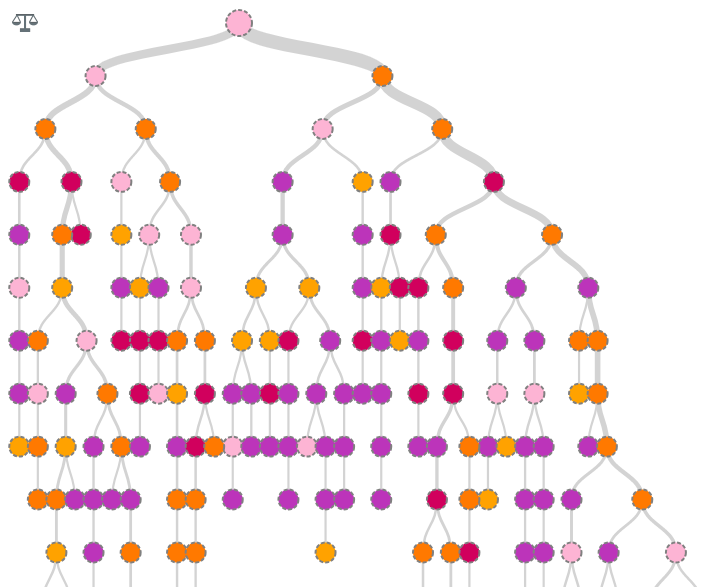
\includegraphics[width=10cm]{ArbAprox1.png}
	\caption{Fragmento de árbol de decisión de la primera aproximación}
	\label{fig:ArbAprox1}
\end{figure}


\subsection{Interpretación (Primera Aproximación)}

Al realizar el \emph{testing} con el resto de los datos (el 30\% restante) obtenemos una matriz de confusión [\ref{fig:ConfMatrixAprox1}], como podemos observar no son datos muy buenos, si bien acertamos el 60\% de los retrasos hay un 40\% que debemos minimizar lo máximo posible ya que el objetivo de nuestro sistema es predecir todos los retrasos, es decir, minimizar los Falsos Negativos. 

\begin{figure}[htb]
	\centering
	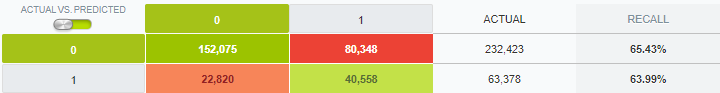
\includegraphics[width=10cm]{ConfMatrixAprox1.png}
	\caption{Matriz de confusión de la primera aproximación}
	\label{fig:ConfMatrixAprox1}
\end{figure}

Pero el objetivo de crear este árbol no era realmente extraer un buen modelo de predicción sino aumentar nuestro conocimiento sobre la importancia de las variables de nuestra tarjeta de datos [\ref{fig:ImportanciaAprox1}]. Podemos ver como la variables más importante es la aerolínea que realiza el vuelo, pero tampoco es un dato excesivamente relevante ya que es un hecho que hay aerolíneas con más retraso que otras. Es decir, nuestro árbol de decisión ha realizado la mayoría de sus predicciones basándose en si ese vuelo lo realizaba una aerolínea con muchos retrasos (los marcaba como 1), o con pocos retrasos (los marcaba como 0).

Otro dato que cobra mucha importancia es el día del verano y las horas programadas de llegada y salida, esto ya nos da unas primeras pistas de que puede existir cierta estacionalidad, por lo que ya empezamos a intuir que una Serie Temporal podría darnos unos mejores resultados.

\begin{figure}[htb]
	\centering
	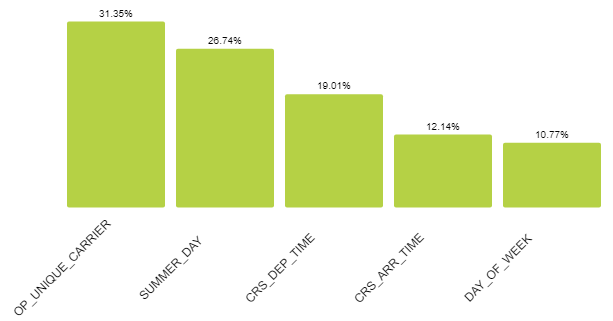
\includegraphics[width=7cm]{ImportanciaAprox1.png}
	\caption{Importancia de las variables de la primera aproximación}
	\label{fig:ImportanciaAprox1}
\end{figure}

\subsection{Minería de Datos (Segunda Aproximación)}

Como una segunda aproximación realizamos otro árbol de decisión [\ref{fig:ArbAprox2}] para hacer una clasificación binaria de forma análoga a la anterior aproximación. En este caso nos quedamos solo con las variables relativas a la hora programada (llegada y salida), con una particularidad, en este caso es una variable categórica que representa el intervalo de tiempo en el que el vuelo se realiza (esta división fue hecha mediante uso de cuantiles para crear una distribución uniforme). Además incluimos el modelo de avión que del vuelo en concreto, por falta de datos referentes al modelo la cantidad de datos se redujo a la mitad, por lo que vimos conveniente empezar a usar todos los datos referentes al año completo, no solo el verano como en la aproximación anterior.

\begin{figure}[htb]
	\centering
	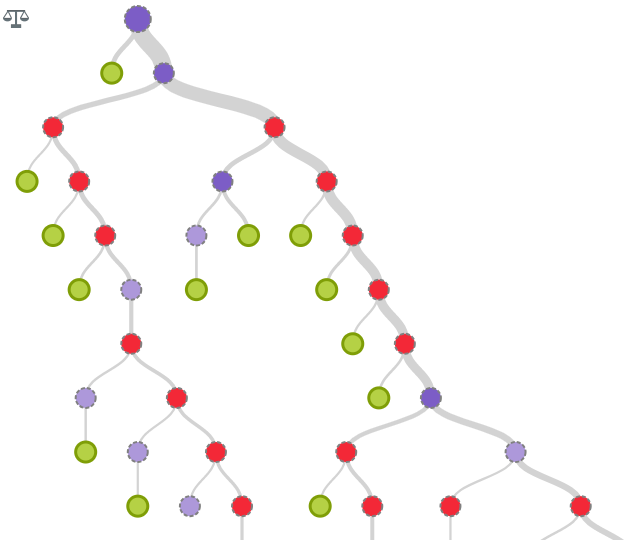
\includegraphics[width=10cm]{ArbAprox2.png}
	\caption{Fragmento de árbol de decisión de la segunda aproximación}
	\label{fig:ArbAprox2}
\end{figure}

\subsection{Interpretación (Segunda Aproximación)}
Como se puede observar en el árbol [\ref{fig:ArbAprox2}] en los nodos de color rojo (modelo de avión), esta es una característica que parece cobrar mucha importancia (esto también se puede ver en [\ref{fig:ImportanciaAprox2}]) en este caso es porque hay ciertos modelos de avión que realizan viajes más cortos y que otros, por lo que en un día pueden realizar muchos viajes y por tanto, acumular más retraso en el caso que se produzca. De nuevo el tiempo vuelve a cobrar cierta importancia por lo antes mencionado.

Los resultados mostrados en la matriz de confusión [\ref{fig:ConfMatrixAprox2}] vuelven a no ser muy buenos, si bien la proporción de falsos negativos se reduce, los falsos positivos aumentan. Aunque dar un falso positivo no es algo crítico, sí que se puede observar un gran exceso de estos y habría que reducirlos, pero no es necesario una minimización de los mismos.

\begin{figure}[htb]
	\centering
	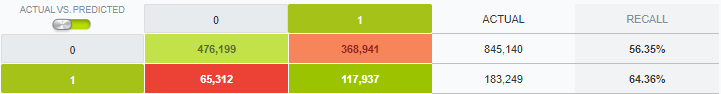
\includegraphics[width=10cm]{ConfMatrixAprox2.png}
	\caption{Matriz de confusión de la primera aproximación}
	\label{fig:ConfMatrixAprox2}
\end{figure}

\begin{figure}[htb]
	\centering
	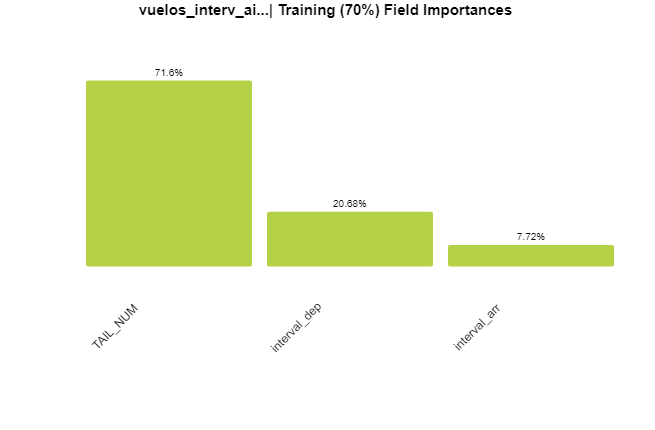
\includegraphics[width=7cm]{ImportanciaAprox2.png}
	\caption{Importancia de las variables de la primera aproximación}
	\label{fig:ImportanciaAprox2}
\end{figure}

%----------------------------------------------------------------------------


%---------------------------------------------------------------------------

\subsection{Regresión}
Una vez terminadas las anteriores aproximaciones destinadas a conseguir clasificar los vuelos entre aquellos que se retrasaron y aquellos que no, con mejor o peor resultado, procedemos a intentar predecir cuanto se retrasará un determinado vuelo.

Para ello, utilizaremos series temporales, en concreto, series temporales regulares. Por este motivo, necesitamos obtener registros que contengan información sobre intervalos de tiempo espaciados regularmente, que en nuestro caso, serán días. Así, obtendremos un nuevo \textit{Dataset}, que contiene 426 registros, dado que estamos utilizando los datos correspondientes a un año completo y dos meses. El retraso correspondiente a cada uno de estos registros será el retraso medio de ese día.

Adicionalmente, utilizaremos los datos correspondientes a un solo modelo de avión. Por ello, ya tenemos nuestros datos para la regresión, los retrasos medios de un modelo de avión en cada día desde Abril de 2017 a Mayo de 2018. Utilizaremos un 90\% de los datos para \emph{training} y un 10\% en \emph{testing}, lo que se corresponde con utilizar los meses el primer año completo, de Abril a Marzo, en \emph{training} y el resto en \emph{testing}. En [\ref{fig:Regresion737}] vemos un ejemplo utilizando los datos del modelo Boeing 737-7H4.

\begin{figure}[htb]
	\centering
	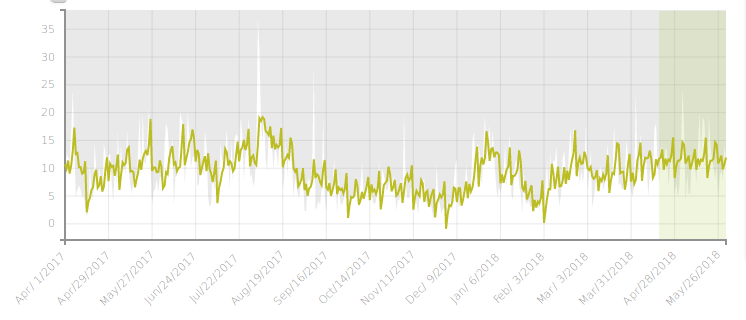
\includegraphics[width=14cm]{Regresion-737.png}
	\caption{Regresión obtenida utilizando los datos del modelo 737-7H4}
	\label{fig:Regresion737}
\end{figure}

Como podemos ver en [\ref{fig:Regresion737}], en la parte derecha (correspondiente a los datos de \emph{testing}), el modelo (en verde) predice correctamente los retrasos, siguiendo los máximos y mínimos reales (en blanco).

Ahora bien, para obtener estos resultados, es decir, predecir correctamente el retraso que tendrá un vuelo, necesitamos tan solo dos datos, el día de dicho vuelo y el modelo de avión que se utilizará. Dado que el modelo de avión podría ser, o no, conocido de antemano, cabe preguntarse si los datos obtenidos utilizando un determinado modelo de avión pueden ser utilizados para otros modelos, considerados similares.

Para ello, utilizaremos los modelos 737-7H4 y 717-200, que bajo nuestro conocimiento del problema cumplen funciones similares. Ambos son aviones comerciales, que transportan pasajeros con su equipaje, y que tienen capacidad para alrededor de 150 pasajeros. Los resultados obtenidos pueden verse en [\ref{fig:Regresion737_2}] y [\ref{fig:Regresion717}]. Los resultados no son prometedores, y queda patente que no sería posible utilizar los datos de un modelo para predecir el retraso de otros modelos distintos.

\begin{figure}[bht]
	\centering
	\begin{subfigure}{\linewidth}
		\centering
		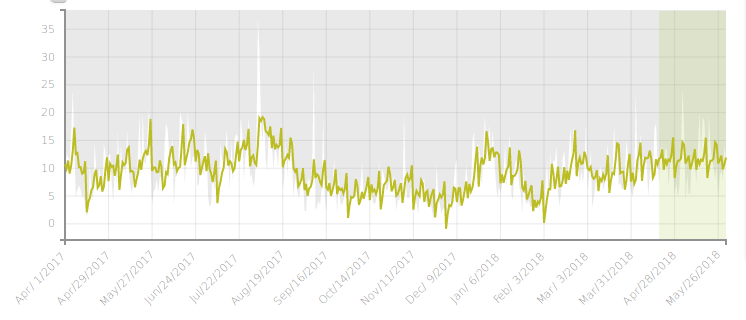
\includegraphics[width=9cm]{Regresion-737.png}
		\caption{Modelo 737-7H4}
		\label{fig:Regresion737_2}
	\end{subfigure}
	\begin{subfigure}{\linewidth}
		\centering
		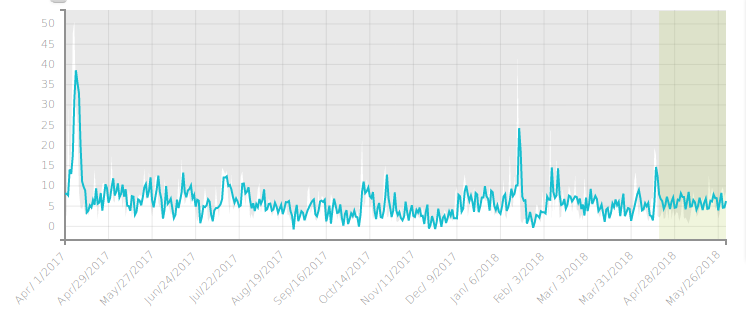
\includegraphics[width=9cm]{Regresion-717.png}
		\caption{Modelo 717-200}
		\label{fig:Regresion717}
	\end{subfigure}
	\caption{Regresión utilizando dos modelos diferentes}
	\label{fig:Regresion_737_717}
\end{figure} 

\section{Conclusiones}

A lo largo de este documento hemos obtenido diversos resultados, en nuestro intento de predecir retrasos en vuelos de avión, en Estados Unidos. Las primeras aproximaciones a clasificar los vuelos entre aquellos con retraso y aquellos sin él, dieron buenos resultados, si bien mejorables. En el caso de la regresión, no se obtuvo ningún resultado satisfactorio.

De cara al futuro, y a mejorar los resultados, consideramos posibles dos mejoras. La primera de ellas es obtener información adicional relativa a los vuelos, como por ejemplo, la climatología. La segunda mejora consiste en aumentar nuestro conocimiento del dominio, que nos permitiría un mejor uso de los datos que ya disponemos.

\end{document}